\documentclass[a4paper]{article}
\usepackage{ctex}
\usepackage{geometry}
\usepackage{amsmath}
\usepackage{ulem}
\usepackage{graphicx}
\usepackage{siunitx}
\usepackage{enumitem}
\usepackage{multirow}
\usepackage{adjustbox}
\usepackage[hidelinks]{hyperref}
\usepackage{tabularx}
\usepackage{array}
\usepackage{float}
\usepackage{caption}
\newcolumntype{Y}{>{\centering\arraybackslash}X}

\geometry{left=2.5cm, right=2.5cm, top=2.5cm, bottom=2.5cm}
\zihao{-4}

\begin{document}

\noindent\textbf{班级：24级整合科学班} \hspace{1cm} \textbf{学号：2400017802} \hspace{1cm} \textbf{姓名：冯翊展} \hspace{1cm} \textbf{评分：}\\
\textbf{同组学生：无} \\
\textbf{实验名称：三极管，运算放大器和发光二极管}   \hfill \textbf{实验日期：2025年5月23日} 

\hrule
\vspace{3mm}

\begin{enumerate}[label=\chinese*.,left=0pt]
    \item 实验目的
    \begin{enumerate}[label=\arabic*.,left=0pt]
        \item 使用三极管的放大功能驱动电磁铁。
        \item 了解运算放大器的特性，搭建反向放大器和非反向放大器电路并测量其增益。
        \item 测量发光二极管的工作曲线，并使用运算放大器室使发光二极管发光。
    \end{enumerate}
    
    \item 基本原理
    \begin{enumerate}[label=\arabic*.,left=0pt]
        \item 三级管
        \\[1mm]
        三极管是一种常用的半导体器件，广泛应用于放大电路和开关电路中。其主要成分为硅或锗单质，按结构形式分为NPN和PNP两种，N型半导体掺杂富电子原子（如磷），P型半导体掺杂缺电子原子（如硼）。三极管有三个引脚，依次为发射极(E)，基极(B)和集电极(C)，相邻两极之间存在一个PN结，称为集电结和发射结。\\[1mm]
        三极管的工作状态分三种。以NPN三极管为例，当基极与发射极之间的电压小于导通电压（$\qty{0.6}{}\sim\qty{0.7}{\V}$）时，三极管各极均无电流，称为截止状态；当基极与发射极之间的电压大于导通电压时，发射结导通，此时集电极电流近似与基极电流成正比，即 $I_C = \beta I_B$ ，放大系数在几十至几百，称为放大状态；继续增大基极电压和电流，集电极电流达到最大值，不再随基极电流增大而增大，此时三极管相当于导通，称为饱和状态。
        \begin{figure}[H]
            \centering
            \scalebox{0.9}{
            \begin{minipage}{0.55\textwidth}
                \centering
                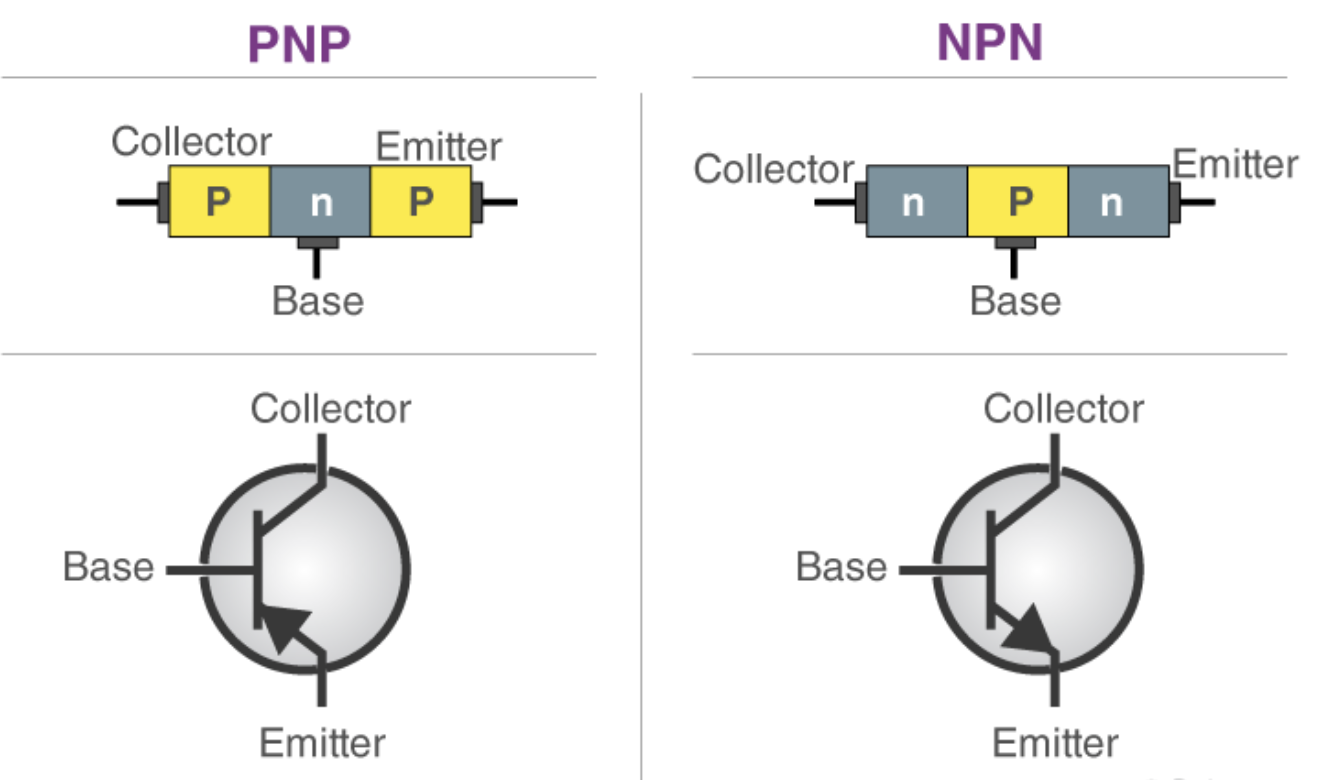
\includegraphics[width=\textwidth]{BJT.png}
            \end{minipage}
            \begin{minipage}{0.43\textwidth}
                \centering
                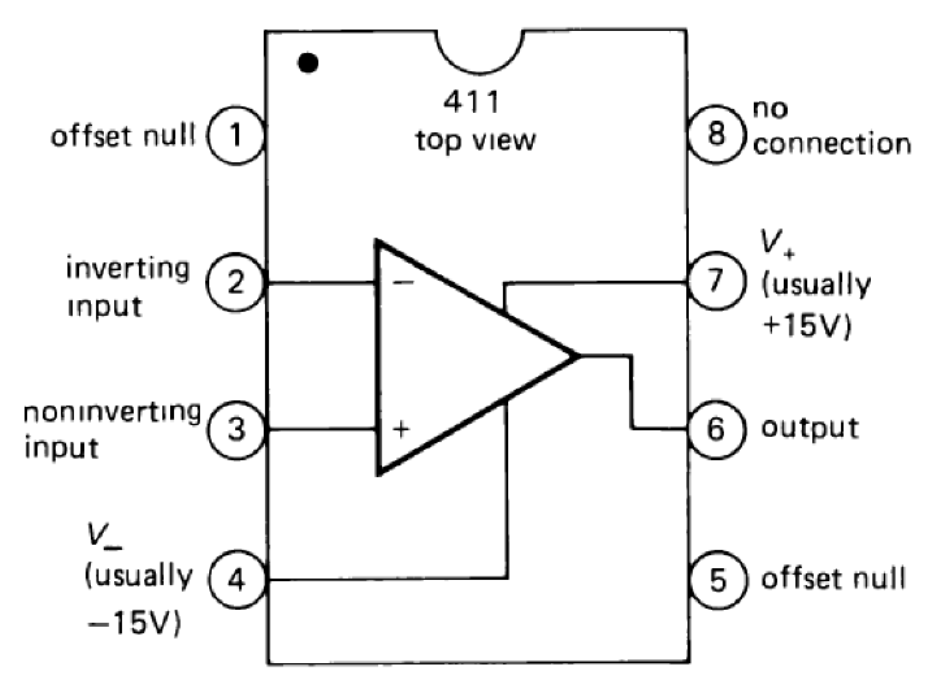
\includegraphics[width=\textwidth]{Op-amp.png}
            \end{minipage}
            }
            \caption{三极管与运算放大器}
        \end{figure}
        

        \item 运算放大器
        \\[1mm]
        运算放大器是一种高增益的电子电路元器件，广泛用于信号放大、比较等模拟电路中。典型的运算放大器有5个主要引脚：反相输入端（-），同相输入端（+），输出端，正电源（+V）和负电源（-V）。理想运算放大器具有的两个核心特性：输入端电流为0（即输入阻抗无限大），以及输入端电压差为0（即 $V_+ = V_-$）。\\[1mm]
        运算放大器可以用于组装电压放大电路，分为反相放大器电路和非反相放大器电路。基于运算放大器的两个特性，由欧姆定律可得其理论放大增益$A_\text{T}$：对于反向放大器 $V_\text{out}/V_\text{in} =−R_2/R_1$，对于非反相放大器 $V_\text{out}/V_\text{in} = 1 + R_2/R_1$。
        \begin{figure}[H]
            \centering
            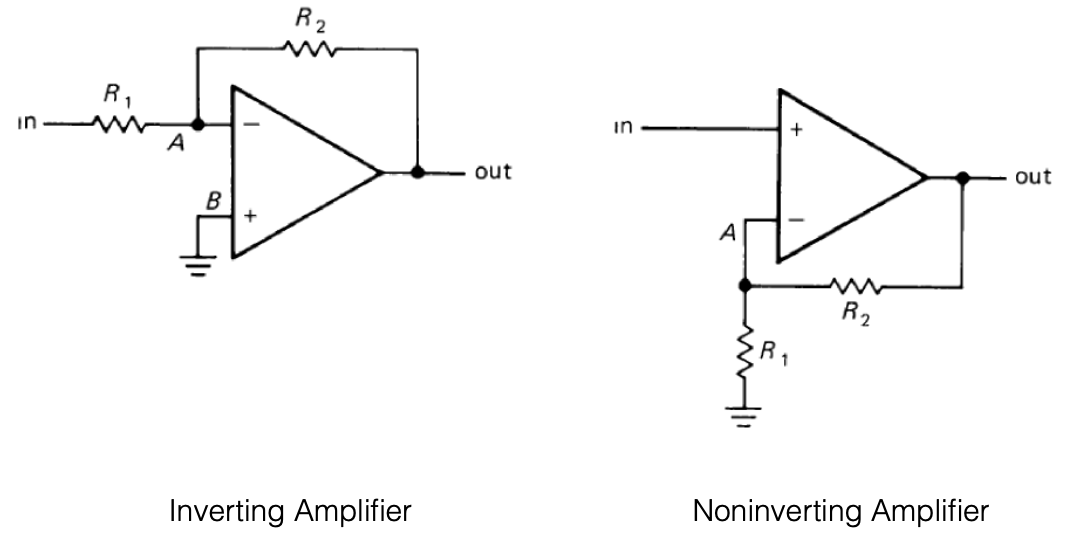
\includegraphics[width=0.6\linewidth]{Amplifier.png}
            \caption{反相与非反相放大器}
        \end{figure}
    \end{enumerate}
    
    \item 仪器与试剂
    \\[3mm]
    面包板，NPN型三极管，LF411CN运算放大器，二极管，发光二极管，电磁铁，定值电阻，电容，万用表，信号发生器，学生电源，导线

    \item 实验步骤
    \begin{enumerate}[label=\arabic*.,left=0pt]
        \item 在面包板上搭建电路，利用三极管和辅助元件实现对电磁铁的控制。
        \item 在面包板上安放LF411运算放大器，为放大器提供 $\qty{\pm15}{\V}$ 供电。将放大器的正输入端接地，调整负输入端电压，测量并记录输出端电压。
        \item 选取两个阻值适当的电阻，搭建非反相放大器电路，测量其实际电压增益并与理论值比较。更换电阻重复测量。再搭建反相放大电路并重复以上实验。
        \item 测量LED工作电流对输入电压的函数关系。
        \item 使用运算放大器连接LED驱动电路，改变输入电压测量LED两端电压。将输入端改为信号发生器，调节信号频率观察LED亮度变化。
    \end{enumerate}
    
    \item 实验结果与分析
    \begin{enumerate}[label=\arabic*.,left=0pt]
        \item 三极管驱动电磁铁
        \begin{figure}[H]
            \centering
            \scalebox{0.8}{
            \begin{minipage}{0.35\textwidth}
                \centering
                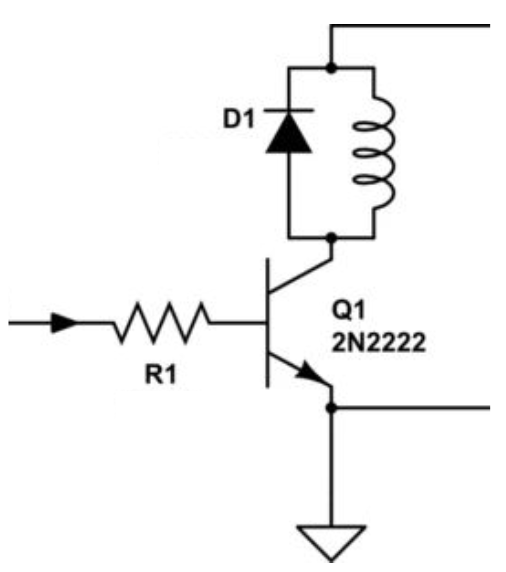
\includegraphics[width=\textwidth]{BJT-Elctromagnet demo.png}
            \end{minipage}
            \begin{minipage}{0.5\textwidth}
                \centering
                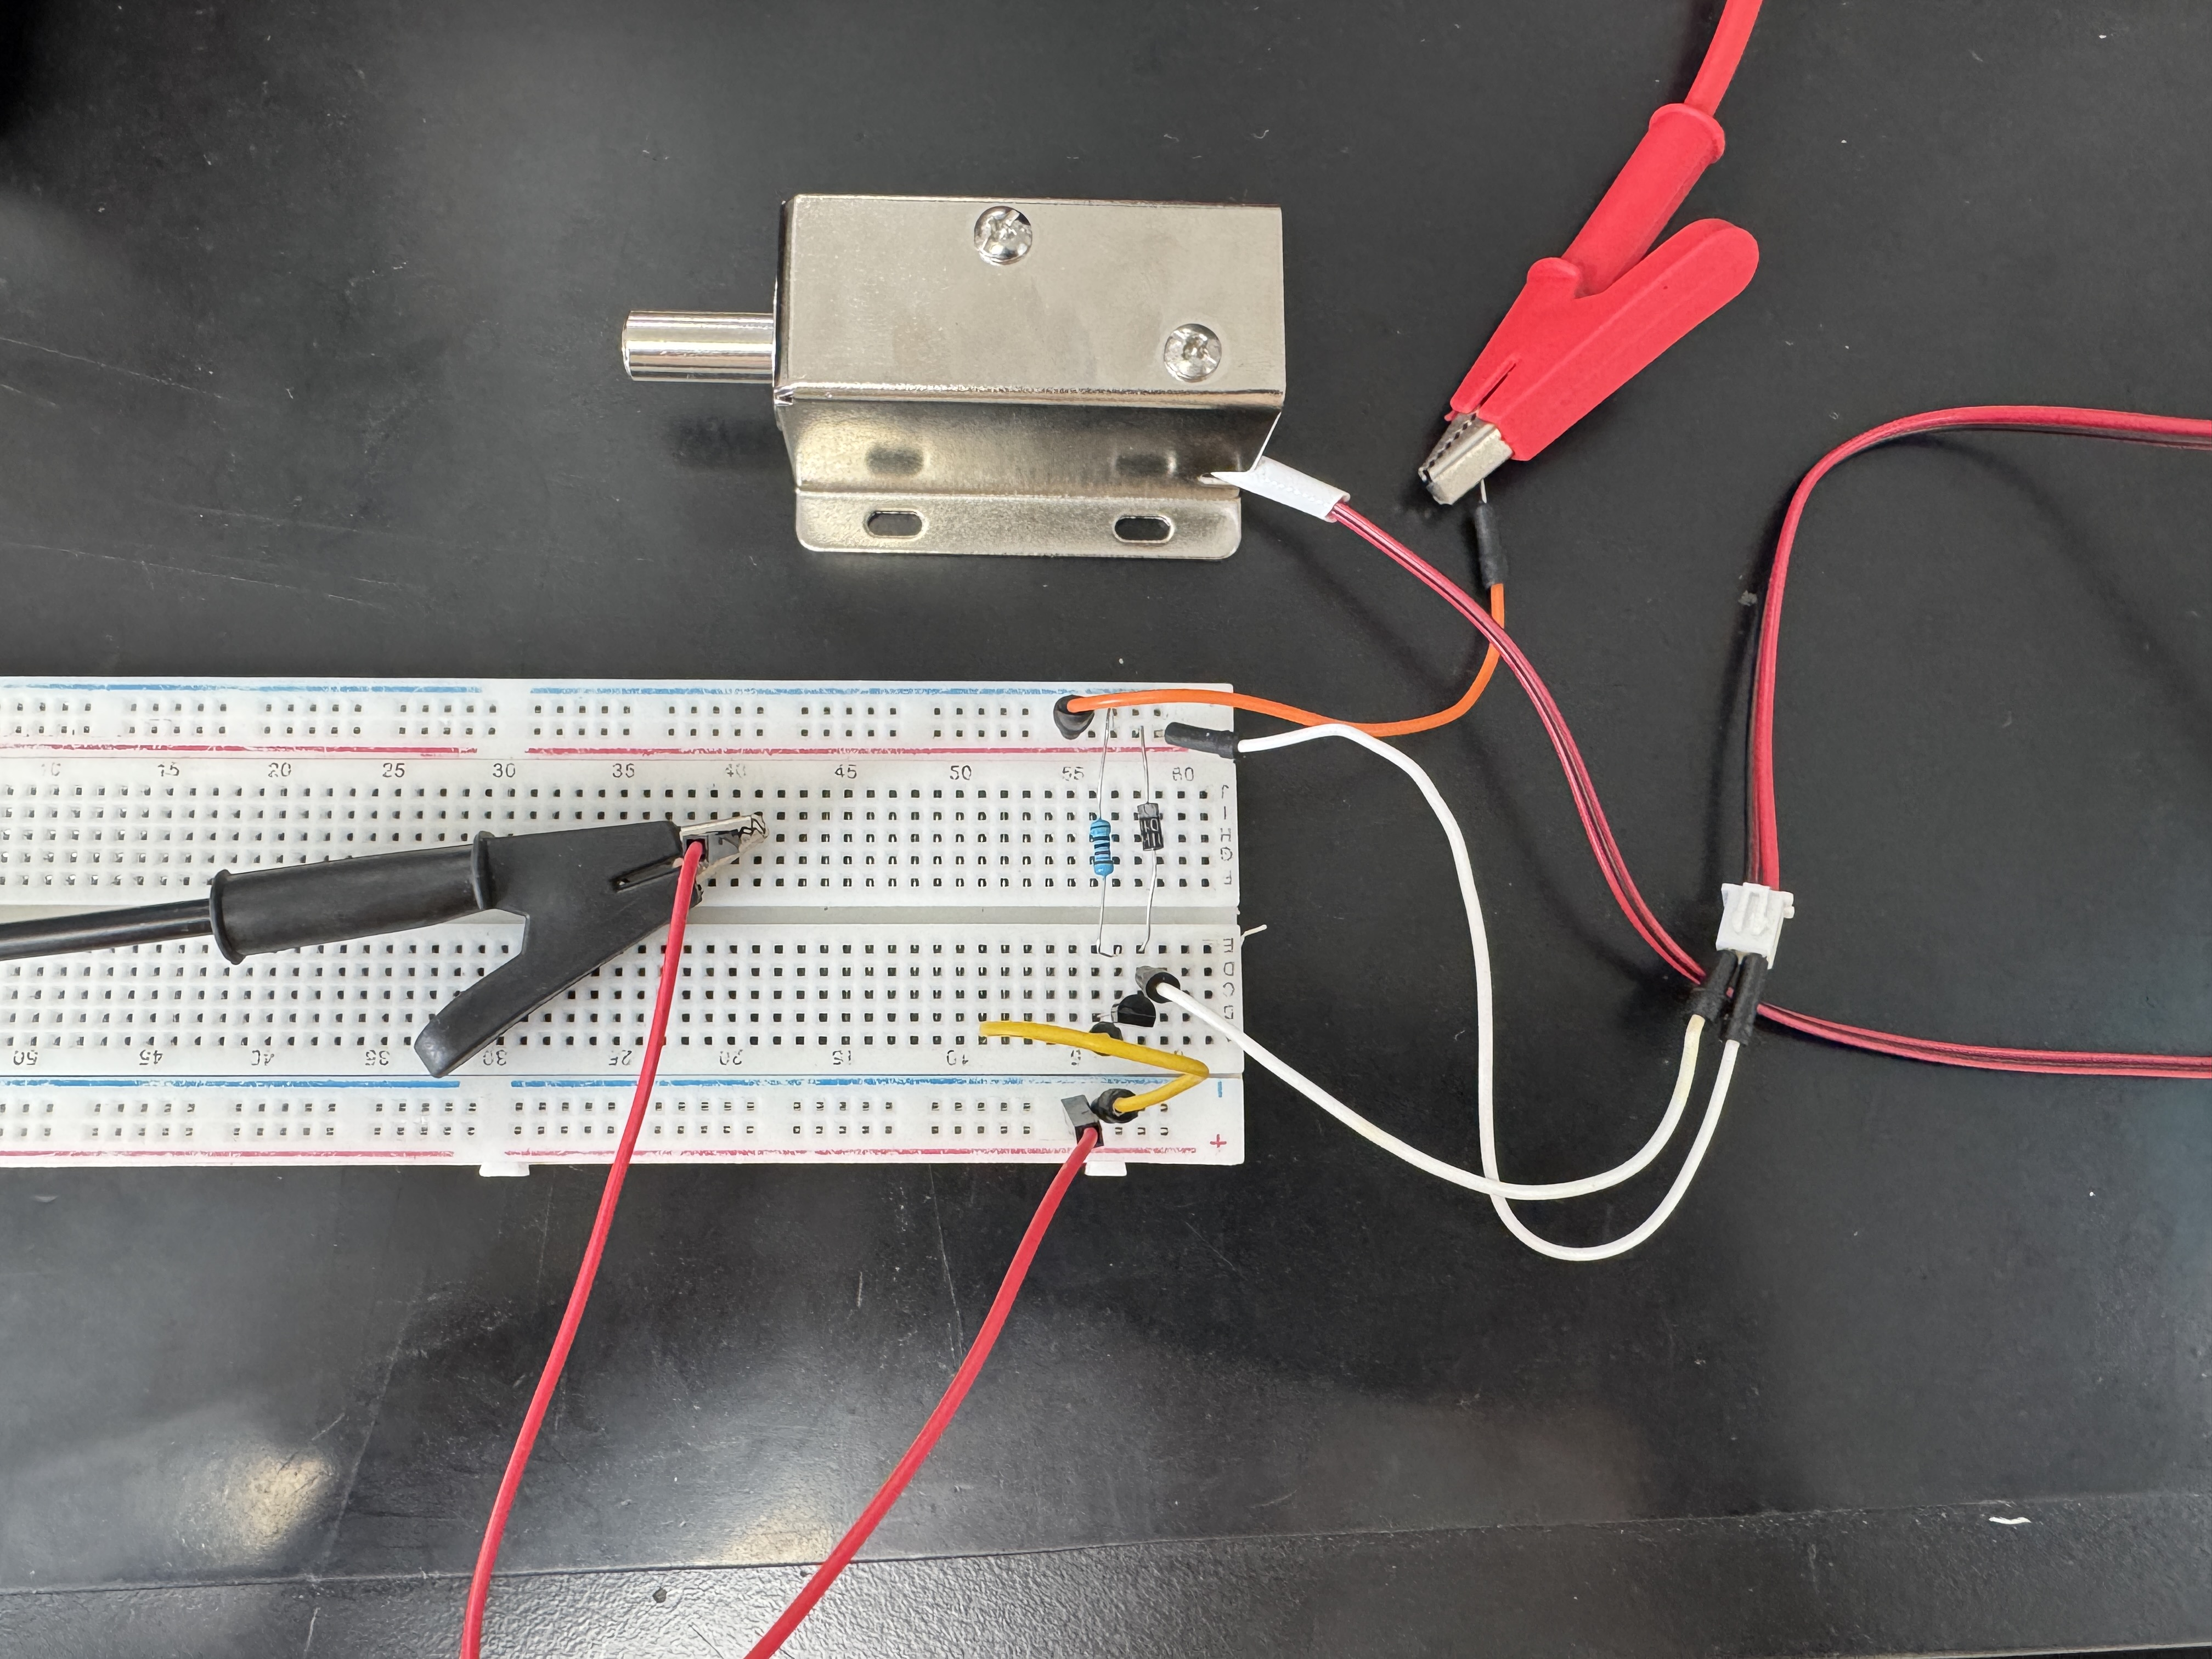
\includegraphics[width=\textwidth]{BJT-Electromagnet.JPG}
            \end{minipage}
            }
            \caption{三极管驱动电磁铁电路}
        \end{figure}
        实验电路如图 3，其中 $R_1=\qty{10.33}{\kohm}$，二极管的目的是保护三极管不被电磁铁的自感电流击穿。实际测得电磁铁平放时，释放电压为 $\qty{3.50}{\V}$，吸附电压为 $\qty{12.5}{\V}$，两者不一致的原因为电磁铁内部还存在摩擦力阻碍金属圆柱运动。

        \item 运算放大器
        \\[1mm]
        首先将运算放大器的正输入端接地，调整负输入端电压，测量得到对应的输出端电压如下：
        \\[-7mm]
        \begin{table}[H]
            \caption{运算放大器输入-输出电压关系}
            \centering
            \scalebox{0.9}{ 
            \setlength{\tabcolsep}{6pt}
            \renewcommand{\arraystretch}{1.2} 
            \begin{tabular}{ccc|ccc}
            $V_+$ & $V_-$ & $V_\text{out}$ & $V_+$ & $V_-$ & $V_\text{out}$  \\ 
            GND   & $\qty{+15}{\V}$ & $\qty{-13.57}{\V}$ & GND & $\qty{-15}{\V}$ & $\qty{+14.32}{\V}$ \\ 
            GND   & $\qty{+10.02}{\V}$ & $\qty{-13.57}{\V}$ & GND & $\qty{-10.00}{\V}$ & $\qty{+14.32}{\V}$ \\ 
            GND   & $\qty{+4.99}{\V}$ & $\qty{-13.57}{\V}$ & GND & $\qty{-4.98}{\V}$ & $\qty{+14.31}{\V}$ \\
            GND   & $\qty{+1.01}{\V}$ & $\qty{-13.57}{\V}$ & GND & $\qty{-1.00}{\V}$ & $\qty{+14.31}{\V}$ \\
            GND   & $\qty{+0.502}{\V}$ & $\qty{-13.55}{\V}$ & GND & $\qty{-0.498}{\V}$ & $\qty{+14.31}{\V}$ \\ 
            GND   & $\qty{+0.003}{\V}$ & $\qty{-13.45}{\V}$ & GND & $\qty{-0.003}{\V}$ & $\qty{+14.30}{\V}$ \\ 
            \end{tabular}
            }
        \end{table}
        
        \vspace{-3mm}
        可以看到，输出电压在负输入端电压的符号改变时出现突变，且在无电阻的情况下，运算放大器的放大倍率很大，可以将 $\qty{}{\mV}$ 级别的电压放大至几乎最大量程。

        \item 反相与非反相放大电路
        \\[1mm]
        选取不同阻值的电阻搭建图2中的反相与非反相放大电路，测量不同 $V_\text{in}$ 输入时的输出电压 $V_\text{out}$，并据此计算实际增益 $A=V_\text{out}/V_\text{in}$ 和理论增益 $A_\text{T}$比较，结果如下：\\[-6mm]
        \begin{minipage}[t]{0.48\linewidth}
        \begin{table}[H]
            \caption{反相放大电路增益}
            \centering
            \scalebox{0.75}{ 
            \setlength{\tabcolsep}{6pt}
            \renewcommand{\arraystretch}{1.2} 
            \begin{tabular}{cccccc}
            $R_1$ & $R_2$ & $V_\text{in}$     & $V_\text{out}$    & $A$  & $A_\text{T}$  \\ 
                  &       & $\qty{1.01}{\V}$ & $\qty{-1.65}{\V}$ & -1.63 &               \\ 
            $\qty{48.8}{\ohm}$ & $\qty{77.4}{\ohm}$ & $\qty{5.12}{\V}$ & $\qty{-8.07}{\V}$ & -1.58 & -1.59 \\ 
                  &       & $\qty{8.02}{\V}$ & $\qty{-12.8}{\V}$ & -1.60 &               \\ 
            \hline
                  &       & $\qty{15.8}{\mV}$ & $\qty{-2.01}{\V}$ & -127 &  \\ 
            $\qty{77.4}{\ohm}$ & $\qty{9.83}{\kohm}$  & $\qty{49.2}{\mV}$ & $\qty{-6.26}{\V}$ & -127 & -127 \\ 
                  &       & $\qty{100.4}{\mV}$ & $\qty{-12.85}{\V}$ & -128 &               \\ 
            \hline
                  &       & $\qty{0.494}{\V}$ & $\qty{-3.792}{\V}$ & -7.68 &               \\ 
            $\qty{9.83}{\kohm}$ & $\qty{75.3}{\kohm}$ & $\qty{0.973}{\V}$ & $\qty{-7.46}{\V}$ & -7.67 & -7.66 \\ 
                  &       & $\qty{1.510}{\V}$ & $\qty{-11.60}{\V}$ & -7.68 &               \\ 
                
            \end{tabular}
            }
        \end{table}
        \end{minipage}
        \hfill
        \begin{minipage}[t]{0.48\linewidth}
        \begin{table}[H]
            \caption{非反相放大电路增益}
            \centering
            \scalebox{0.75}{ 
            \setlength{\tabcolsep}{6pt}
            \renewcommand{\arraystretch}{1.2} 
            \begin{tabular}{cccccc}
            $R_1$ & $R_2$ & $V_\text{in}$     & $V_\text{out}$    & $A$  & $A_\text{T}$  \\ 
                  &       & $\qty{0.101}{\V}$ & $\qty{0.263}{\V}$ & 2.60 &               \\ 
            $\qty{48.8}{\ohm}$ & $\qty{77.4}{\ohm}$ & $\qty{0.502}{\V}$ & $\qty{1.308}{\V}$ & 2.61 & 2.59 \\ 
                  &       & $\qty{1.001}{\V}$ & $\qty{2.561}{\V}$ & 2.56 &               \\ 
            \hline
                  &       & $\qty{14.9}{\mV}$ & $\qty{1.888}{\V}$ & 127 &               \\ 
            $\qty{77.4}{\ohm}$ & $\qty{9.83}{\kohm}$ & $\qty{51.7}{\mV}$ & $\qty{6.62}{\V}$ & 128 & 128 \\ 
                  &       & $\qty{0.101}{\V}$ & $\qty{13.01}{\V}$ & 129 &               \\ 
            \hline
                  &       & $\qty{0.509}{\V}$ & $\qty{4.41}{\V}$ & 8.66 &               \\ 
            $\qty{9.83}{\kohm}$ & $\qty{75.3}{\kohm}$ & $\qty{1.002}{\V}$ & $\qty{8.68}{\V}$ & 8.66 & 8.66 \\ 
                  &       & $\qty{1.511}{\V}$ & $\qty{13.10}{\V}$ & 8.67 &               \\ 
                 
                
            \end{tabular}
            }
        \end{table}
        \end{minipage}
        \\[3mm]

        可以看到，电路的实际增益与理论增益基本一致，当选取电阻阻值较小时误差最大，这可能是运算放大器内部存在的阻抗所导致的。

        \item LED电流-电压特性曲线
        \\[1mm]
        发光二极管（LED）是一种能够将电能转化为光能的半导体器件，具有特殊的电流-电压特性曲线（图4左）。将LED与万用表串联接入电路，测量外加电压为 $\qty{2}{} \sim \qty{3.8}{\V}$ 区间内相应的电流大小并绘图（图4右）。观察发现，当外加电压低于 $\qty{2.8}{\V} $时，流经LED的电流很微弱，LED几乎不发光；外加电压为$\qty{2.8}{} \sim \qty{3.2}{\V}$ 时，LED微亮；外加电压高于 $\qty{3.2}{\V}$ 时，LED发出强亮光。

        \item LED 控制电路
        \\[1mm]
        搭建LED控制电路如图5，其中电位器用于调节正相输入端的输入电压，从而间接调节负相输入端的电压；正负电源接入处并联两个电容器，用于滤去电流中的交流杂波。首先接入$\qty{15}{\V}$的直流电源，调节电位器，测量LED两端电压并用ImageJ分析LED发光强度，结果如表4。
        \begin{figure}[H]
            \centering
            \scalebox{0.75}{
            \begin{minipage}{0.45\textwidth}
                \centering
                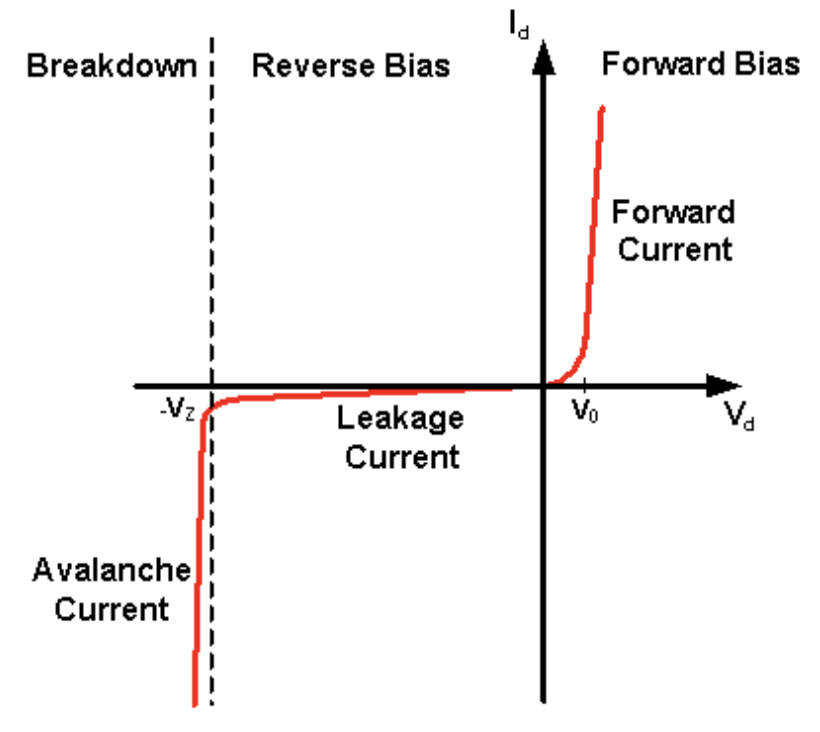
\includegraphics[width=\textwidth]{LED I-V Curve.png}
            \end{minipage}
            \begin{minipage}{0.54\textwidth}
                \centering
                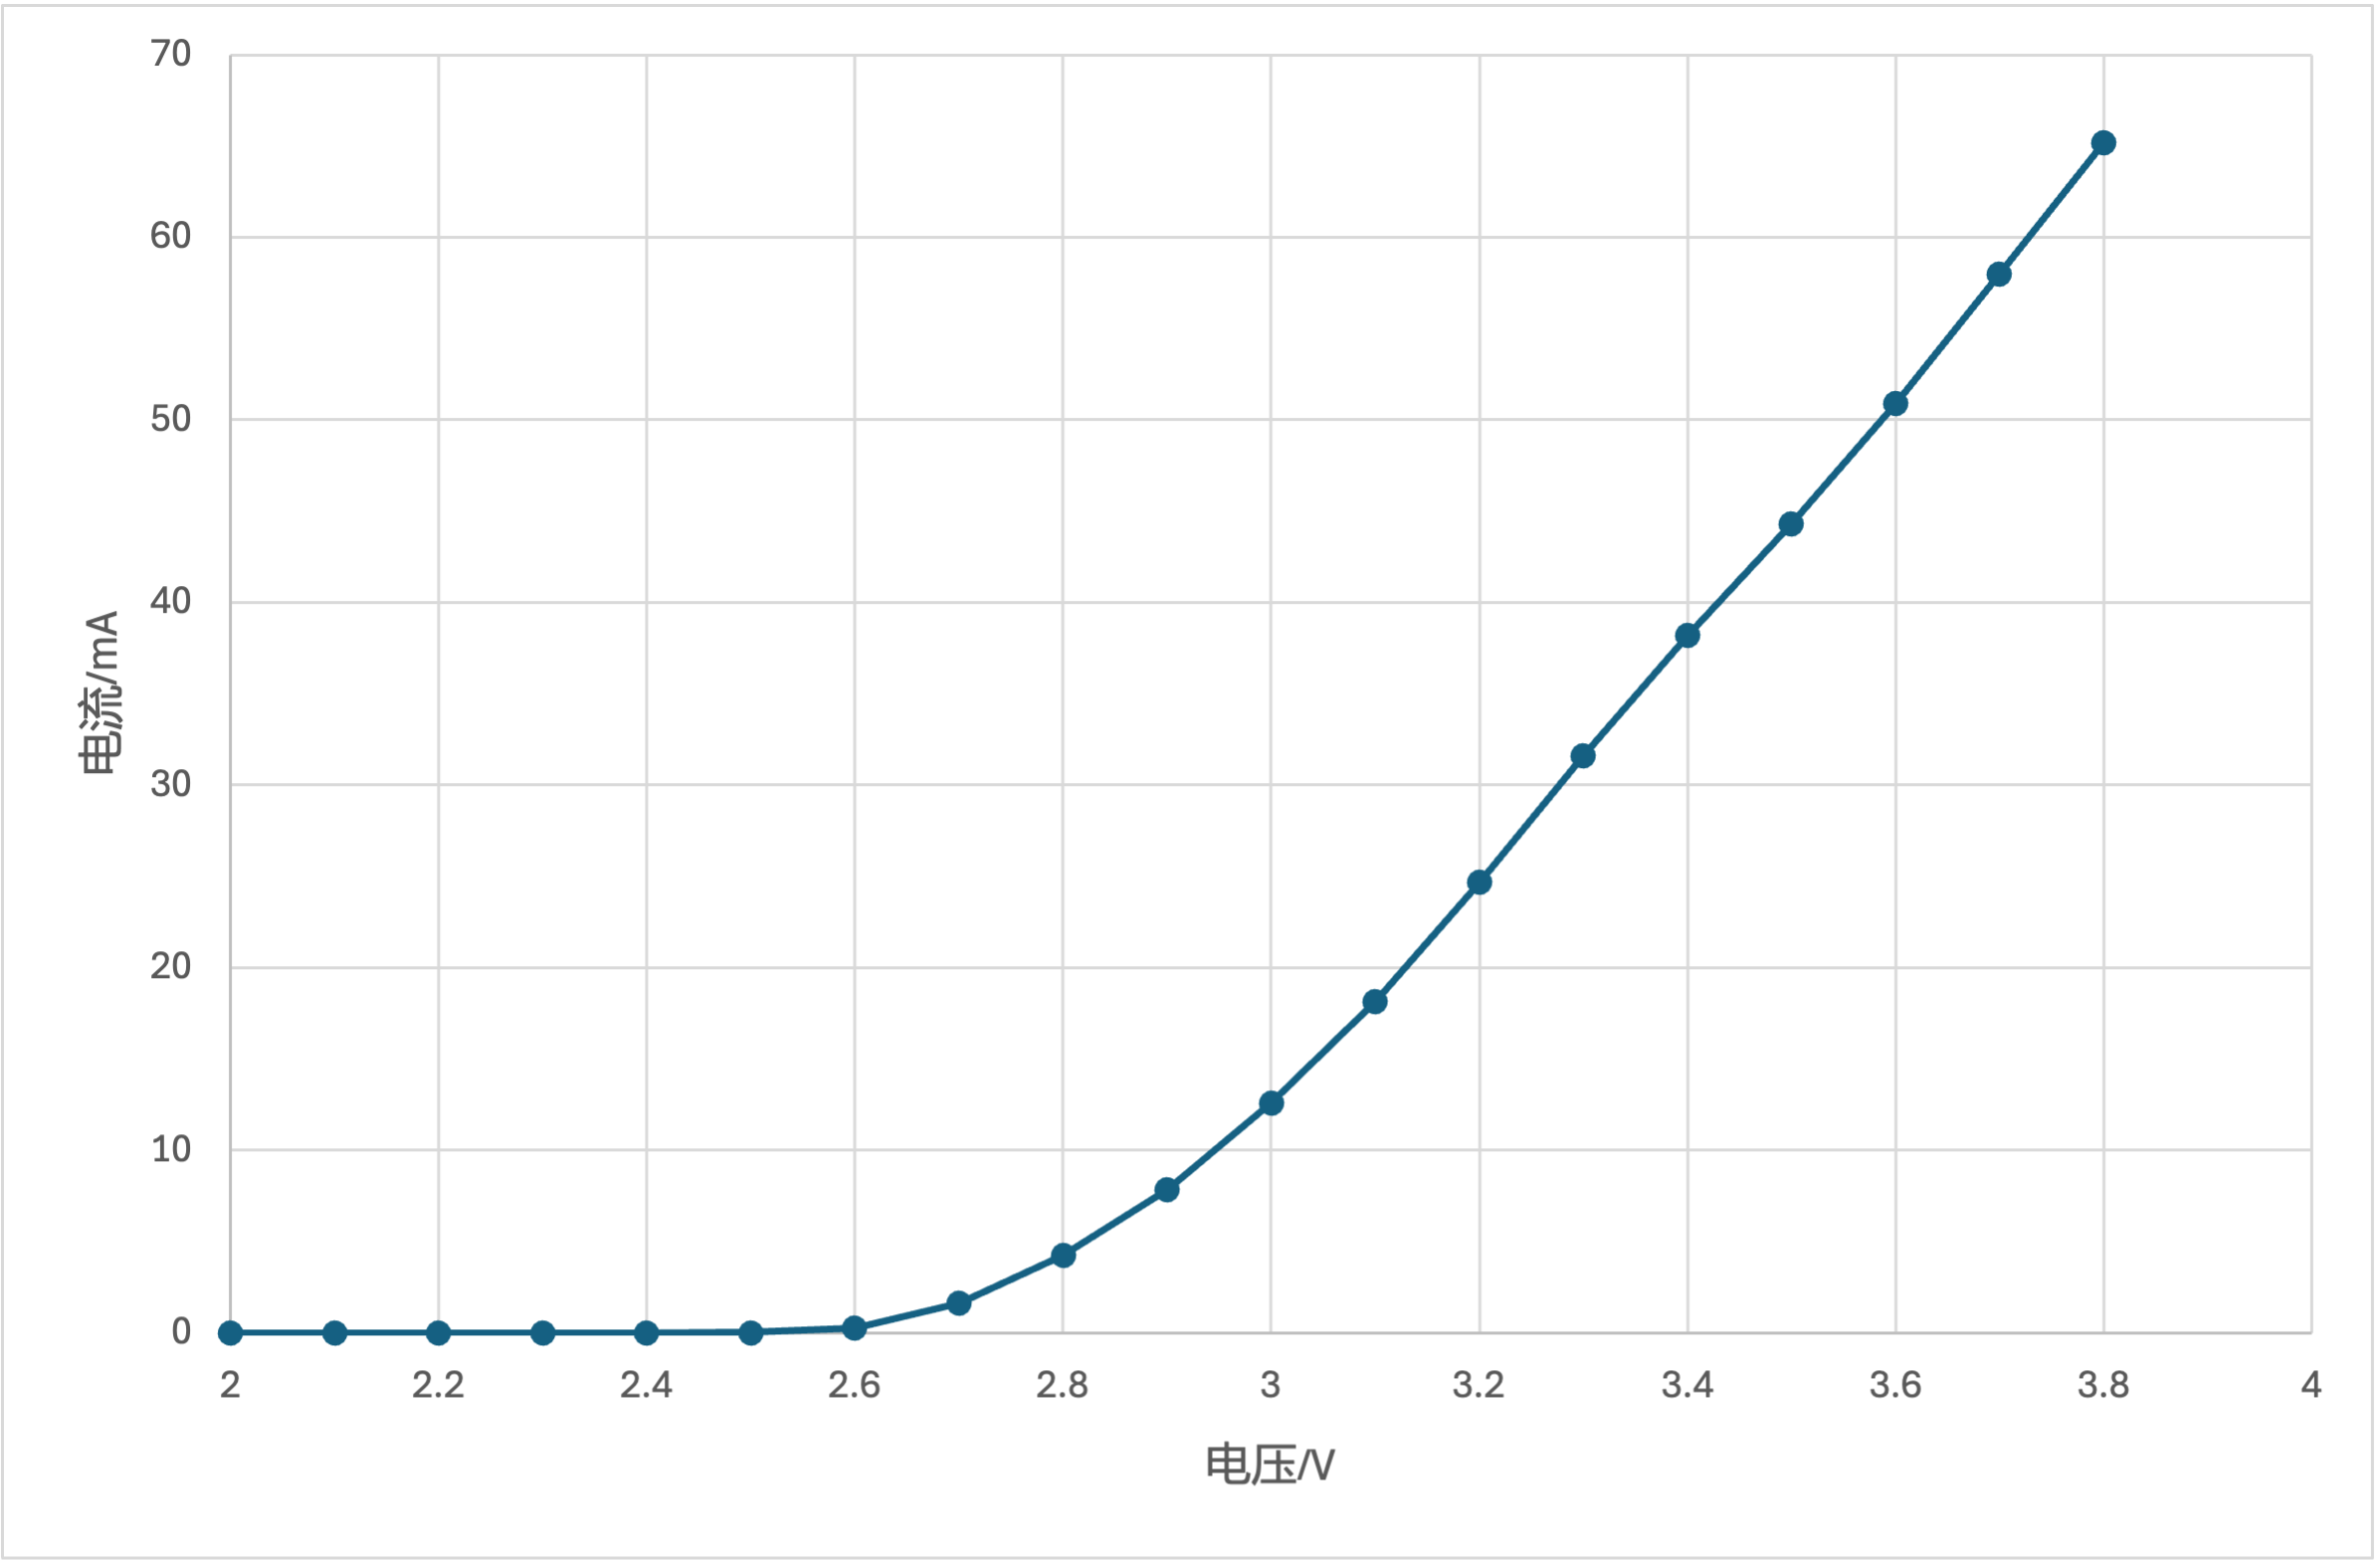
\includegraphics[width=\textwidth]{LED I-V Curve d.png}
            \end{minipage}
            }
            \caption{LED电流-电压特性曲线}
        \end{figure}
        
        \begin{figure}[H]
            \centering
            \scalebox{}{
            \begin{minipage}{0.4\textwidth}
                \centering
                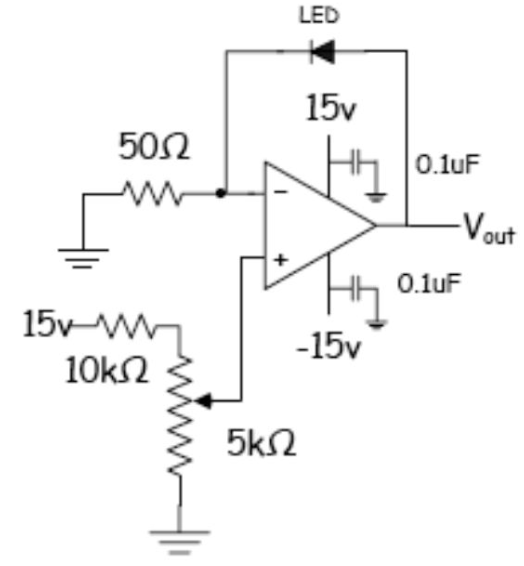
\includegraphics[width=0.8\linewidth]{LED_Control Circuit.png}
                \captionof{figure}{LED控制电路}
            \end{minipage}
            \begin{minipage}{0.5\textwidth}
                \begin{table}[H]
                    \caption{非反相放大电路增益}
                    \centering
                    \scalebox{1}{ 
                    \setlength{\tabcolsep}{10pt}
                    \renewcommand{\arraystretch}{1.2} 
                    \begin{tabular}{ccc}
                    $V_\text{LED}$    & 灰度 & 相对亮度\\
                    $\qty{2.534}{\V}$ & 216.7 & 0 \\
                    $\qty{2.649}{\V}$ & 221.9 & +5.2 \\
                    $\qty{2.742}{\V}$ & 240.2 & +23.5 \\
                    $\qty{2.827}{\V}$ & 250.3 & +33.6 \\
                    $\qty{2.936}{\V}$ & 254.6 & +37.9 \\
                    $\qty{3.059}{\V}$ & 254.6 & +37.9 \\
                    $\qty{3.080}{\V}$ & 254.6 & +37.9 \\
                    \end{tabular}
                    }
                \end{table}
            \end{minipage}
            }
        \end{figure}
        可以看到，使用运算放大器控制LED，LED两端电压有上限，当电压接近 $\qty{3}{\V}$ 时，LED达到最大发光其强度。\\[1mm]
        将直流电源换为信号发生器，输入信号为 $\qty{0.1}{} \sim \qty{60}{\Hz}$的正弦波。当输入正弦波的频率在 $\qty{0.1}{} \sim \qty{1}{\Hz}$ 时，可以清晰地观察到LED亮度周期性的变亮-变暗的过程；当输入正弦波的频率在 $\qty{5}{} \sim \qty{30}{\Hz}$ 时，观察到LED在快速闪烁，且闪烁频率与输入正弦波频率一致；当输入正弦波的频率达到 $\qty{60}{\Hz}$ 时，肉眼已无法到LED亮度变化。

        \item 误差分析
        \\[1mm]
        本实验的主要误差来源于万用表以及运算放大器等元件的内部阻抗。另外，在测量电压时，运算放大器电路容易出现周期性的扰动，使得测量电压不稳定，产生一定测量误差。
        
    \end{enumerate}
\end{enumerate}
\end{document}